\begin{figure}[htbp]
			\centering
			\resizebox{\textwidth}{!}{%
				\begin{tikzpicture}[
					trave/.style={line width=1.8pt, line cap=round, line join=round, black},
					terra/.style={line width=0.8pt, black},
					diag/.style={line width=0.90pt, black},
					nodoV/.style={circle, fill=white, draw=black,
						inner sep=0pt, minimum size=5.0pt, line width=0.80pt},
					segno/.style={circle, draw=black, fill=white, inner sep=0pt,
						minimum size=8pt, font=\tiny, line width=0.55pt},
					etlab/.style={circle, draw=black, line width=0.6pt,
						fill=white, inner sep=2pt, font=\small},
					lab/.style={font=\small},
					]
					
					\def\L{1.80}
					\def\SEP{5.80}
					\def\dNo{0.55}
					\def\dTo{0.30}
					\def\dMo{0.75}
					
					\def\portale{\draw[trave](0,0)--(0,\L)--(2*\L,\L)--(2*\L,0);}
					\def\cernieraA{%
						\draw[terra](0,0)--(-0.24,-0.40)--(0.24,-0.40)--cycle;
						\draw[terra](-0.34,-0.40)--(0.34,-0.40);
						\foreach \x in {-0.28,-0.16,-0.04,0.08,0.20,0.30}
						\draw[very thin](\x,-0.40)--++(-0.08,-0.11);
						\node[nodoV]at(0,0){};}
					\def\cernieraB{%
						\draw[terra](2*\L,0)--(2*\L-0.24,-0.40)--(2*\L+0.24,-0.40)--cycle;
						\draw[terra]({2*\L-0.34},-0.40)--({2*\L+0.34},-0.40);
						\foreach \x in {-0.28,-0.16,-0.04,0.08,0.20,0.30}
						\draw[very thin]({2*\L+\x},-0.40)--++(-0.08,-0.11);
						\node[nodoV]at(2*\L,0){};}
					
					%%═══ PANNELLO (a) — N₂ ═════════════════════════════════════════════════
					%% Specchio di N₁: col.sin=trazione(+) interno, col.des=compressione(-) esterno
					%%                 traverso=compressione(-) sotto
					\begin{scope}[xshift=0cm]
						%% Col. sin.: trazione (+), interno (destra di AC)
						\fill[gray!15](0,0)--(\dNo,0)--(\dNo,\L)--(0,\L)--cycle;
						\foreach \y in {0.15,0.30,...,1.75}{\draw[gray!50,very thin](0,\y)--(\dNo,\y);}
						\draw[diag](\dNo,0)--(\dNo,\L);
						\draw[diag](0,0)--(\dNo,0);
						\draw[diag](0,\L)--(\dNo,\L);
						%% Col. des.: compressione (-), esterno (destra di BD)
						\fill[gray!15](2*\L,0)--({2*\L+\dNo},0)--({2*\L+\dNo},\L)--(2*\L,\L)--cycle;
						\foreach \y in {0.15,0.30,...,1.75}{\draw[gray!50,very thin](2*\L,\y)--({2*\L+\dNo},\y);}
						\draw[diag]({2*\L+\dNo},0)--({2*\L+\dNo},\L);
						\draw[diag](2*\L,0)--({2*\L+\dNo},0);
						\draw[diag](2*\L,\L)--({2*\L+\dNo},\L);
						%% Traverso: compressione (-), sopra (evita sovrapposizione con col.sin)
						\fill[gray!15](0,\L)--(2*\L,\L)--(2*\L,{\L+\dNo})--(0,{\L+\dNo})--cycle;
						\foreach \x in {0.35,0.70,...,3.50}{\draw[gray!50,very thin](\x,\L)--(\x,{\L+\dNo});}
						\draw[diag](0,{\L+\dNo})--(2*\L,{\L+\dNo});
						\draw[diag](0,\L)--(0,{\L+\dNo});
						\draw[diag](2*\L,\L)--(2*\L,{\L+\dNo});
						\portale \cernieraA \cernieraB
						%% Trattini mancanti: bordo sup. del rettangolo di col.sin (coperto dalla trave)
						%% Ridisegnati 0.06 cm sopra il centro-trave, dove sono visibili sul fondo grigio
						\draw[diag](\dNo,\L)--(\dNo,{\L+0.06});       % prolungamento bordo destro
						\node[nodoV]at(\L,\L){};
						\node[segno]at(\dNo/2,{\L*0.50}){$+$};
						\node[segno]at({2*\L+\dNo/2},{\L*0.50}){$-$};
						\node[segno]at({0.5*\L},{\L+\dNo/2}){$-$};
						\node[segno]at({1.5*\L},{\L+\dNo/2}){$-$};
						\node[right=0.04,lab]at(\dNo,{\L*0.50}){$\tfrac{1}{2\ell}$};
						\node[right=0.04,lab]at({2*\L+\dNo},{\L*0.50}){$\tfrac{1}{2\ell}$};
						\node[above=0.04,lab]at(\L,{\L+\dNo}){$\tfrac{1}{2\ell}$};
						\node[left,lab]at(0,0){$A$};
						\node[left,lab]at(2*\L,0){$B$};
						\node[above left,lab]at(0,\L){$C$};
						\node[above right,lab]at(2*\L,\L){$D$};
						\node[above,lab]at(\L,\L){$M$};
						\node[etlab]at(\L,{0}){$N_2$};
					\end{scope}
					
					%%═══ PANNELLO (b) — T₂ ═════════════════════════════════════════════════
					%% Specchio di T₁: col.sin=(-) esterno, col.des=(+) esterno, traverso=(-) sotto
					\begin{scope}[xshift=\SEP cm]
						%% Col. sin.: (-), esterno (sinistra di AC)
						\fill[gray!15]({-\dTo},0)--(0,0)--(0,\L)--({-\dTo},\L)--cycle;
						\foreach \y in {0.15,0.30,...,1.75}{\draw[gray!50,very thin]({-\dTo},\y)--(0,\y);}
						\draw[diag]({-\dTo},0)--({-\dTo},\L);
						\draw[diag]({-\dTo},0)--(0,0);
						\draw[diag]({-\dTo},\L)--(0,\L);
						%% Col. des.: (+), esterno (destra di BD)
						\fill[gray!15](2*\L,0)--({2*\L+\dTo},0)--({2*\L+\dTo},\L)--(2*\L,\L)--cycle;
						\foreach \y in {0.15,0.30,...,1.75}{\draw[gray!50,very thin](2*\L,\y)--({2*\L+\dTo},\y);}
						\draw[diag]({2*\L+\dTo},0)--({2*\L+\dTo},\L);
						\draw[diag](2*\L,0)--({2*\L+\dTo},0);
						\draw[diag](2*\L,\L)--({2*\L+\dTo},\L);
						%% Traverso: (-), sotto
						\fill[gray!15](0,{\L-\dTo})--(2*\L,{\L-\dTo})--(2*\L,\L)--(0,\L)--cycle;
						\foreach \x in {0.35,0.70,...,3.50}{\draw[gray!50,very thin](\x,{\L-\dTo})--(\x,\L);}
						\draw[diag](0,{\L-\dTo})--(2*\L,{\L-\dTo});
						\portale \cernieraA \cernieraB
						\node[nodoV]at(\L,\L){};
						\node[segno]at({-\dTo/2},{\L*0.50}){$-$};
						\node[segno]at({2*\L+\dTo/2},{\L*0.50}){$+$};
						\node[segno]at({0.5*\L},{\L-\dTo/2}){$-$};
						\node[segno]at({1.5*\L},{\L-\dTo/2}){$-$};
						\node[left=0.04,lab]at({-\dTo},{\L*0.50}){$\tfrac{1}{2\ell}$};
						\node[right=0.04,lab]at({2*\L+\dTo},{\L*0.50}){$\tfrac{1}{2\ell}$};
						\node[below=0.04,lab]at(\L,{\L-\dTo}){$\tfrac{1}{2\ell}$};
						\node[right,lab]at(0,0){$A$};
						\node[left,lab]at(2*\L,0){$B$};
						\node[above,lab]at(0,\L){$C$};
						\node[above,lab]at(2*\L,\L){$D$};
						\node[above,lab]at(\L,\L){$M$};
						\node[etlab]at(\L,{0}){$T_2$};
					\end{scope}
					
					%%═══ PANNELLO (c) — M₂ ═════════════════════════════════════════════════
					%% Specchio di M₁:
					%%   col.sin = triangolo interno destra (0 in A, 1/2 in C)  ← specchio col.des di M₁
					%%   col.des = trapezio esterno destra (1 in B, 1/2 in D)   ← specchio col.sin di M₁
					%%   trav.sin = triangolo sotto (1/2 in C, 0 in M)          ← specchio trav.des di M₁
					%%   trav.des = triangolo sopra (0 in M, 1/2 in D)          ← specchio trav.sin di M₁
					\begin{scope}[xshift={2*\SEP cm}]
						%% M col. sin. (positivo, triangolo a destra di AC — fibra tesa interna)
						\fill[gray!15](0,0)--(0,\L)--(\dMo/2,\L)--cycle;
						\begin{scope}
							\clip(0,0)--(0,\L)--(\dMo/2,\L)--cycle;
							\foreach \y in {0.15,0.30,...,1.75}
							{\draw[gray!50,very thin]({-0.1},\y)--(\dMo/2+0.1,\y);}
						\end{scope}
						\draw[diag](0,0)--(\dMo/2,\L);         % faccia inclinata
						\draw[diag](\dMo/2,\L)--(0,\L);         % chiusura in C (coperta dalla trave)
						%% M col. des. (negativo, trapezio a destra di BD — fibra tesa esterna)
						\fill[gray!15](2*\L,0)--({2*\L+\dMo},0)--({2*\L+\dMo/2},\L)--(2*\L,\L)--cycle;
						\begin{scope}
							\clip(2*\L,0)--({2*\L+\dMo},0)--({2*\L+\dMo/2},\L)--(2*\L,\L)--cycle;
							\foreach \y in {0.15,0.30,...,1.75}
							{\draw[gray!50,very thin](2*\L-0.1,\y)--({2*\L+\dMo+0.1},\y);}
						\end{scope}
						\draw[diag]({2*\L+\dMo},0)--({2*\L+\dMo/2},\L);   % faccia inclinata
						\draw[diag](2*\L,0)--({2*\L+\dMo},0);              % base
						\draw[diag]({2*\L+\dMo/2},\L)--(2*\L,\L);          % chiusura in D (coperta)
						%% M traverso metà sin. (positivo, triangolo sotto: 1/2 in C, 0 in M)
						\fill[gray!15](0,\L)--(0,{\L-\dMo/2})--(\L,\L)--cycle;
						\begin{scope}
							\clip(0,\L)--(0,{\L-\dMo/2})--(\L,\L)--cycle;
							\foreach \x in {0.25,0.50,...,1.75}
							{\draw[gray!50,very thin](\x,{\L-\dMo/2-0.1})--(\x,{\L+0.1});}
						\end{scope}
						\draw[diag](0,{\L-\dMo/2})--(\L,\L);
						\draw[diag](0,{\L-\dMo/2})--(0,\L);     % chiusura in C (coperta dalla colonna)
						%% M traverso metà des. (negativo, triangolo sopra: 0 in M, 1/2 in D)
						\fill[gray!15](\L,\L)--(2*\L,{\L+\dMo/2})--(2*\L,\L)--cycle;
						\begin{scope}
							\clip(\L,\L)--(2*\L,{\L+\dMo/2})--(2*\L,\L)--cycle;
							\foreach \x in {1.90,2.15,...,3.55}
							{\draw[gray!50,very thin](\x,{\L-0.1})--(\x,{\L+\dMo/2+0.1});}
						\end{scope}
						\draw[diag](\L,\L)--(2*\L,{\L+\dMo/2});
						\draw[diag](2*\L,{\L+\dMo/2})--(2*\L,\L);   % chiusura in D (visibile: sopra trave)
						%% Archetto in C: trav.sin (sotto) → col.sin (interno destra)
						\draw[diag](0,{\L-\dMo/2}) arc(270:360:\dMo/2);
						%% Archetto in D: col.des (esterno destra) → trav.des (sopra)
						\draw[diag]({2*\L+\dMo/2},\L) arc(0:90:\dMo/2);
						%% Struttura
						\portale \cernieraA \cernieraB
						\node[nodoV]at(\L,\L){};
						%% Valori
						\node[above,lab]at(\dMo/2,\L){$\tfrac{1}{2}$};
						\node[right=0.04,lab]at({2*\L+\dMo},0){$1$};
						\node[right=0.04,lab]at({2*\L+\dMo/2},\L){$\tfrac{1}{2}$};
						\node[left=0.04,lab]at(0,{\L-\dMo/2}){$\tfrac{1}{2}$};
						\node[above=0.04,lab]at(2*\L,{\L+\dMo/2}){$\tfrac{1}{2}$};
						%% Etichette nodi
						\node[left,lab]at(0,0){$A$};
						\node[left,lab]at(2*\L,0){$B$};
						\node[above left,lab]at(0,\L){$C$};
						\node[below left,lab]at(2*\L,\L){$D$};
						\node[below=0.04,lab]at(\L,\L){$M$};
						\node[etlab]at(\L,{0}){$M_2$};
					\end{scope}
					
				\end{tikzpicture}
			}%
			\caption{Autosoluzione~$2$ ($\chi_2 = 1$, coppia unitaria in~$B$):
				diagrammi di $N_2$, $T_2$ e $M_2$ sul portale a tre cerniere.
				Gli archetti in~$C$ e ~$D$ indicano la continuità del momento flettente
				ai due nodi rigidi.}
			\label{fig:portale_autosoluzione2}
		\end{figure}
